\section{Zielsetzung}
\label{sec:Zielsetzung}
Ziel dieses Versuches ist es den Wärmetransport entgegen des Temperaturgradienten zu untersuchen. 
Dafür werden Merkmale wie die Güteziffer und der Massendurchsatz und deren Qualität bestimmt.

\section{Theorie}
\label{sec:Theorie}
Der zweite Hauptsatz der Thermodynamik besagt in diesem Zusammenhang, dass Wärme von einem wärmeren Reservoir in das Kältere fließt.
Dieser Prozess kann auch umgekehrt werden, zum Beispiel, wie in diesem Versuch, mit der Wärmepumpe.
Für diese Umkehrung wird Arbeit benötigt, was im Folgenden näher erklärt wird.\\ 
In \autoref{fig:Wärmepumpe_theo} ist der prinzipielle Aufbau einer Wärmepumpe gegeben, wobei $p_b>p_a$ und $T_1>T_2$ gilt.
\begin{figure}[H]
    \centering
    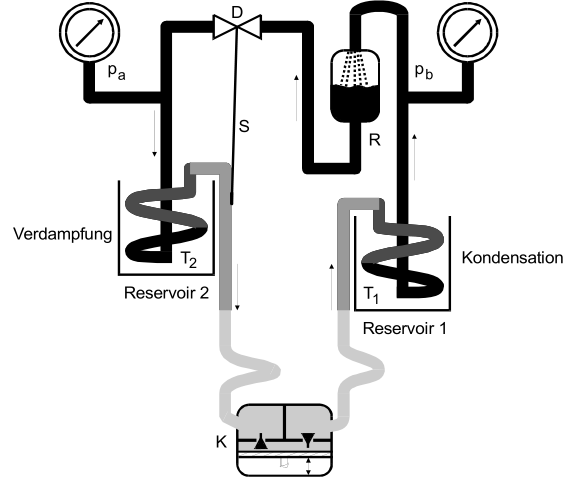
\includegraphics[width=0.6\textwidth]{build/Abb1.png}
    \caption{Prinzipieller Aufbau einer Wärmepumpe \cite[196]{V206}.}
    \label{fig:Wärmepumpe_theo}
\end{figure}


\subsection{Güteziffer} % (fold)
\label{sub:Güteziffer}
Die Güteziffer $\nu$ beschreibt das Verhältnis der transportierten Wärmemenge und der dafür aufgewandten Arbeit $A$ im idealisierten Fall.
So gilt für die Güteziffer einer idealen Wärmepumpe
\begin{equation}
    \nu_{ideal} = \frac{Q_1}{A} = \frac{T_1}{T_1 - T_2}
    \label{eqn:Güteziffer_ideal}
\end{equation} 
und für die reale Wärmepumpe
\begin{equation*}
    \nu_{real} < \frac{T_1}{T_1 - T_2}.
\end{equation*}
$Q_1$ steht für die abgegebene Wärmemenge . 
Nach dem ersten Hauptsatz der Wärmelehre gilt für die abgegebene Wärmemenge
\begin{equation*}
    Q_1 = Q_2 + A ,
\end{equation*}
wobei $Q_2$  die entnommene Wärmemenge ist.
Eine weitere wichtige Beziehung für die Wärmemengen lässt sich aus dem zweiten Hauptsatz der Wärmelehre herleiten.
Für den idealen Fall gilt
\begin{align*}
    \frac{Q_1}{T_1}-\frac{Q_2}{T_2} = 0,\\
    \intertext{wenn die Wärmeübertragung reversibel ist. Für den realen, irreversiblen Teil gilt}\\
    \frac{Q_1}{T_1}-\frac{Q_2}{T_2} > 0.
\end{align*}
Zur Berechnung von der realen Güteziffer wird im Folgenden 
\begin{equation}
    \nu_{real} = \frac{\Delta Q_1}{\Delta t \bar{N}}
    \label{eqn:Güteziffer}
\end{equation}
benutzt. 
$\bar{N}$ ist die vom Wattmeter angezeigte und über das Zeitintervall $\Delta t$ gemittelte Leistungsaufnahme des Kompressors.
Für $\frac{\Delta Q_1}{\Delta t}$ wird
\begin{equation}
    \frac{\Delta Q_1}{\Delta t} = (m_1 c_w + m_k c_k)\frac{\Delta T_1}{\Delta t}
    \label{eqn:DeltaQ1}
\end{equation}
eingesetzt, wobei $m_1 c_w$ die Wärmekapazität des Wassers im Reservoir 1 ist und $m_k c_k$ ist die Wärmekapazität der Kupferschlange und des Eimers.
% subsection Güteziffer (end)
 \subsection{Massendurchsatz} % (fold)
 \label{sub:Massendurchsatz}
 Die Wärmemenge 
 \begin{equation}
     \frac{\Delta Q_2}{\Delta t} = (m_2 c_w + m_k c_k)\frac{\Delta T_2}{\Delta t},
     \label{eqn:DeltaQ2}
 \end{equation}
die pro Zeiteinheit aus dem Reservoir 2 entnommen wird,
wird mit der Verdampfungswärme $L$, die pro Zeit- und Masseneinheit verbraucht wird, gleichgesetzt
\begin{equation}
    \frac{\Delta Q_2}{\Delta t} = L \frac{\Delta m}{\Delta t}.
    \label{eqn:Ldm}
\end{equation}
Um den Massendurchsatz bestimmen zu können wird die \autoref{eqn:Ldm} nach
\begin{equation}
    \frac{\Delta m}{\Delta t} = (m_2 c_w + m_k c_k)\frac{\Delta T_2}{\Delta t} \frac{1}{L}
    \label{eqn:Massendurchsatz}
\end{equation}
umgestellt.
 % subsection Massendurchsatz (end)

\subsection{Die mechanische Kompressorleistung} % (fold)
\label{sub:Die mechanische Kompressorleistung}
Die Arbeit 
 \begin{equation*}
     A_m = - \int_{V_a}^{V_b} p dV
 \end{equation*}
wird allgemein von dem Kompressor geleistet, wenn dieser ein Gasvolumen $V_a$ auf $V_b$ verringert.
Es wird angenommen, das die Kompression adiabatisch ist, sodass die Poissonsche Gleichung 
 \begin{equation*}
     p_a V_a^{\kappa} = p_b V_b^{\kappa} = p V^{\kappa}
 \end{equation*}
angewendet werden kann.
Mit den beiden Formeln ergibt sich die mechanische Kompressorleistung zu
\begin{equation}
    N_{mech} = \frac{\Delta A_m}{\Delta t} = \frac{1}{\kappa - 1} \Bigl(p_b \sqrt[\kappa]{\frac{p_a}{p_b}}-p_a \Bigr) \frac{1}{\rho}\frac{\Delta m}{\Delta t},
    \label{eqn:Kompressorleistung}
\end{equation}
mit der Dichte $\rho$ beim Druck $p_a$.
 % subsection Die mechanische Kompressorleistung (end)